\documentclass[varwidth=40cm]{standalone}
\usepackage{tikz}
\usepackage{pgfplots}
\usepackage{style}

\begin{document}
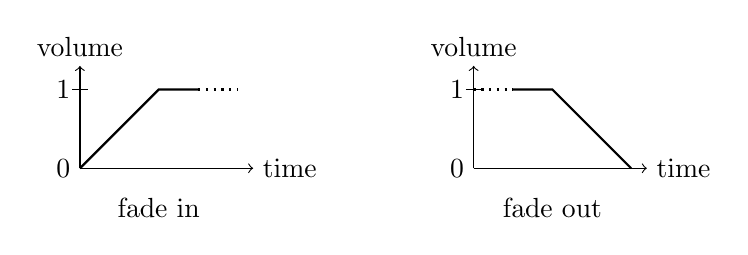
\begin{tikzpicture}
  \draw[->] (0,0) -- (2.2,0) node[right] {time};
  \draw[->] (0,0) -- (0,1.3) node[above] {volume};
  \draw (-.1,1) -- (.1,1);
  \draw (0,0) node[left] {0};
  \draw (0,1) node[left] {1};
  \draw[thick] (0,0) -- (1,1) -- (1.5,1);
  \draw[thick,dotted] (1.5,1) -- (2,1);
  \draw(1,-.5) node {fade in};

  \begin{scope}[shift={(5,0)}]
    \draw[->] (0,0) -- (2.2,0) node[right] {time};
    \draw[->] (0,0) -- (0,1.3) node[above] {volume};
    \draw (-.1,1) -- (.1,1);
    \draw (0,0) node[left] {0};
    \draw (0,1) node[left] {1};
    \draw[thick] (.5,1) -- (1,1) -- (2,0);
    \draw[thick,dotted] (0,1) -- (.5,1);
    \draw(1,-.5) node {fade out};
  \end{scope}
\end{tikzpicture}
\end{document}
